\documentclass[11pt,letterpaper]{article}
\usepackage[margin=0.9in,headheight=14pt]{geometry}
\usepackage{amsmath,amssymb}
\usepackage{enumitem}
\usepackage{fancyhdr}
\usepackage{lmodern}
\usepackage[T1]{fontenc}
\usepackage[dvipsnames]{xcolor}
\usepackage[most]{tcolorbox}
\usepackage{booktabs}
\usepackage{pgfplots}
\usetikzlibrary{arrows.meta,positioning,shapes.geometric}
\pgfplotsset{
  compat=1.18,
  every axis/.append style={grid=major, grid style={gray!25}, tick label style={font=\footnotesize},
    label style={font=\small}, title style={font=\small}, legend style={font=\scriptsize}},
}
\definecolor{cA}{HTML}{1F77B4}
\definecolor{cB}{HTML}{FF7F0E}
\definecolor{cC}{HTML}{2CA02C}
\definecolor{cD}{HTML}{D62728}
\definecolor{cE}{HTML}{9467BD}

\pagestyle{fancy}
\fancyhf{}
\lhead{SYDE 556/750 \qquad Theory guide}
\rhead{Recurrent dynamics (Lecture 6)}
\cfoot{\thepage}
\renewcommand{\headrulewidth}{0pt}

\setlength{\parindent}{0pt}
\setlength{\parskip}{5pt}

\newcommand{\tin}{\tau_{\mathrm{in}}}

\newtcolorbox{key}{colback=Green!6,colframe=Green!50!black,boxrule=0.5pt,left=5pt,right=5pt,top=3pt,bottom=3pt,arc=1pt,fonttitle=\bfseries\small,title=Key idea}
\newtcolorbox{howto}{colback=blue!3,colframe=blue!40!black,boxrule=0.4pt,left=5pt,right=5pt,top=3pt,bottom=3pt,arc=1pt,fonttitle=\bfseries\small,title=How to picture it}
\newtcolorbox{trap}{colback=red!4,colframe=red!50!black,boxrule=0.4pt,left=5pt,right=5pt,top=3pt,bottom=3pt,arc=1pt,fonttitle=\bfseries\small,title=Common trap}

\setlist[enumerate]{leftmargin=1.6em,itemsep=3pt}
\setlist[itemize]{leftmargin=1.4em,itemsep=2pt}

\begin{document}

\begin{center}
{\LARGE\bfseries Recurrent dynamics, from one equation}\\[4pt]
{\large A theory guide to Lecture 6 and the PN3 ramp practice}
\end{center}

\subsection*{How to read this}

Everything in Lecture 6 comes from one fact about synapses. Section~1 states that fact. Each later section either chooses what to feed the synapse to get a behaviour you want, or works out what happens when that input is slightly wrong. Read the sections in order the first time. Afterwards, Section~12 is a one-page summary to revise from.

The ramp sections each part supports:

\begin{center}
\begin{tabular}{@{}ll@{}}
\toprule
This guide & Ramp practice \\
\midrule
1--2 \ The synapse and the loop & 8, 9 \\
3 \ Linear feedback & 10 \\
4 \ Phase portraits & 11 \\
5 \ Designing a system: $A' = \tau A + I$ & 12 \\
6 \ The ideal integral & 13 \\
7 \ Why integrators drift & 14 \\
8 \ Unequal synapses & 15 \\
9 \ Leaky integrators & 16 \\
10 \ Oscillators & 17 \\
11 \ Nonlinear systems and the controlled integrator & 18, 19 \\
\bottomrule
\end{tabular}
\end{center}

%=====================================================================
\section{The one fact: a synapse chases its input}

Let $z(t)$ be whatever arrives at a synapse, and $y = h * z$ what comes out, with the exponential synapse $h(t) = \frac{1}{\tau}e^{-t/\tau}$. Then
\[
\boxed{\ \tau\,\dot y = z - y\ }
\]
\textbf{Why.} $y(t) = \int_{-\infty}^{t}\frac1\tau e^{-(t - t')/\tau}z(t')\,dt'$. Differentiating, the upper limit contributes $\frac1\tau z(t)$, and differentiating the exponential contributes $-\frac1\tau y(t)$. So $\dot y = (z - y)/\tau$.

The Laplace route gives the same thing: $H(s) = \frac{1}{1 + s\tau}$, so $Y(1 + s\tau) = Z$, and $s \to d/dt$ gives $\tau\dot y = z - y$.

\begin{howto}
The output moves toward the input at a speed proportional to how far apart they are. If $z$ jumps to a new value, $y$ covers $63\%$ of the gap in one $\tau$ and $95\%$ in $3\tau$. If $z$ is removed, $y$ decays back to zero with time constant $\tau$.

Two names for the same behaviour: a \emph{low-pass filter} (it smooths fast changes) and a \emph{leaky integrator} (it accumulates its input, $\dot y \propto z$, but leaks away its own value, the $-y$ term).
\end{howto}

\begin{center}
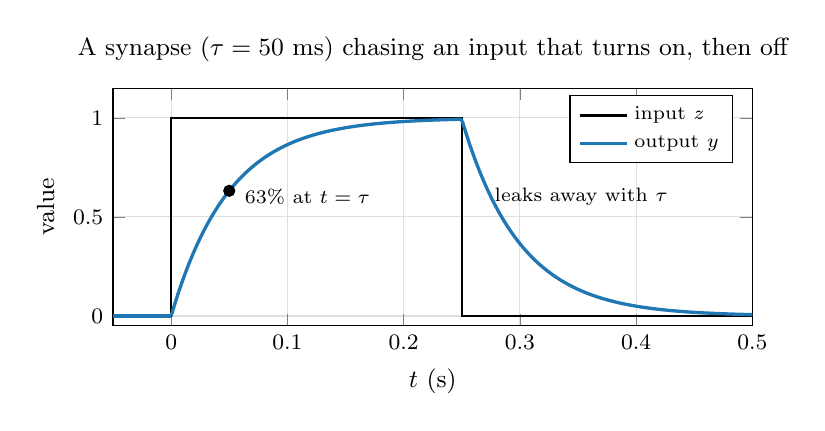
\begin{tikzpicture}
\begin{axis}[width=0.8\textwidth, height=4.6cm, xmin=-0.05, xmax=0.5, ymin=-0.05, ymax=1.15,
  xlabel={$t$ (s)}, ylabel={value}, legend pos=north east, legend cell align=left,
  title={A synapse ($\tau = 50$ ms) chasing an input that turns on, then off}]
  \addplot[black, thick] coordinates {(-0.05,0) (0,0) (0,1) (0.25,1) (0.25,0) (0.5,0)};
  \addplot[cA, very thick, domain=0:0.5, samples=300] {(x<0.25)*(1-exp(-x/0.05)) + (x>=0.25)*(1-exp(-0.25/0.05))*exp(-(x-0.25)/0.05)};
  \addplot[cA, very thick, forget plot] coordinates {(-0.05,0) (0,0)};
  \legend{input $z$, output $y$}
  \addplot[only marks, mark=*, black, forget plot] coordinates {(0.05,0.632)};
  \node[font=\scriptsize, anchor=west] at (axis cs:0.055,0.6) {$63\%$ at $t = \tau$};
  \node[font=\scriptsize, anchor=west] at (axis cs:0.27,0.6) {leaks away with $\tau$};
\end{axis}
\end{tikzpicture}
\end{center}

%=====================================================================
\section{The neural loop}

A population represents $x$. It receives $g(u)$ from an input connection and $f(x)$ from a connection onto itself, both through the same synapse. So the synapse's input is $z = g(u) + f(x)$, and its output is $x$. Put those into Section~1:
\[
\boxed{\ \tau\dot x = \underbrace{g(u) + f(x)}_{z\ \text{(what we feed it)}} - \underbrace{x}_{\text{the leak}}\ }
\]

\begin{key}
This is the \emph{neural loop equation}. Every question in Lecture 6 starts by writing it down, deciding what $z$ is, and simplifying. The $-x$ is always present: it is the synapse leaking. A recurrent connection is the only way to put something back in to oppose it.
\end{key}

\textbf{Why a feed-forward network forgets.} Without the recurrent connection, $f = 0$ and $\tau\dot x = g(u) - x$. When the input stops, $\tau\dot x = -x$, so $x$ decays to zero within a few $\tau$ (tens of milliseconds). Nothing is fed back to oppose the leak.

\textbf{Why the algebraic guess fails.} Writing $x = g(u) + f(x)$ (as Lecture 6 first tries) is only the condition $\dot x = 0$, the place where the state would sit still. It says nothing about how fast the state gets there, or whether it gets there at all. For $f(x) = x + 1$ it even reduces to $0 = u + 1$, which is nonsense as a statement about $x$. The differential equation is the real description.

%=====================================================================
\section{Linear feedback: forget, remember, or explode}

Take $g(u) = u$ and $f(x) = kx$. The loop gives $\tau\dot x = u - (1 - k)x$. The quantity that matters is $1 - k$, \emph{the leak that is left over}: the synapse leaks $x$, and the feedback puts $kx$ back. For a unit step from $x(0) = 0$:
\[
x(t) = \frac{1}{1 - k}\Bigl(1 - e^{-(1-k)t/\tau}\Bigr), \qquad \text{steady state } \frac{1}{1-k}, \quad \text{time constant } \frac{\tau}{1-k}.
\]

\begin{center}
\begin{tabular}{@{}lll@{}}
\toprule
Feedback gain & Left-over leak $1 - k$ & Behaviour \\
\midrule
$k < 1$ & positive & settles at $u/(1-k)$ with time constant $\tau/(1-k)$: \textbf{forgets} \\
$k = 1$ & zero & $\tau\dot x = u$: an integrator, \textbf{remembers} \\
$k > 1$ & negative & grows exponentially until the neurons saturate: \textbf{explodes} \\
\bottomrule
\end{tabular}
\end{center}

\textbf{Quick check.} Plug in $k = -1$: steady state $\tfrac12$, time constant $\tau/2$. This matches Lecture~6's ``converges to $u/2$''. The feedback $-x$ doubles the leak, so the loop is twice as fast as the synapse alone.

The $k = 1$ case is the limit of the formula: $e^{-\epsilon t/\tau} \approx 1 - \epsilon t/\tau$ for small $\epsilon = 1 - k$, so $x \to t/\tau$. The steady state and the time constant both go to infinity together.

%=====================================================================
\section{Phase portraits: reading behaviour off a graph}

When $f$ is nonlinear you usually cannot solve for $x(t)$. You don't need to. In one dimension, $\dot x = \phi(x)$ already tells you which way the state moves at every $x$.

\subsection*{The five steps}
\begin{enumerate}
\item \textbf{Write the loop.} $\phi(x) = \frac1\tau\bigl(u + f(x) - x\bigr)$ with $u$ held at a number. Don't drop the $-x$.
\item \textbf{Equilibria} are where $\phi(x) = 0$: the $x$-intercepts. There the state stops changing.
\item \textbf{Directions.} Where $\phi > 0$, $x$ increases (moves right). Where $\phi < 0$, $x$ decreases (moves left). Draw arrows on the $x$-axis.
\item \textbf{Stability.} Arrows pointing in from both sides: stable. Pointing away: unstable. Shortcut: $\phi'(x^*) < 0$ is stable and $\phi'(x^*) > 0$ is unstable. If $\phi'(x^*) = 0$, the shortcut cannot decide, so use the arrows.
\item \textbf{Behaviour.} From any start, follow the arrow to the next stable equilibrium. If there is none in that direction, the state runs off until the neurons saturate.
\end{enumerate}

\begin{trap}
The state does not slide along the curve, and the bottom of the curve is not an equilibrium. The curve is the state's \emph{velocity}. Its height at each $x$ says how fast and in which direction $x$ is changing. The state itself only moves along the $x$-axis.
\end{trap}

\textbf{Example} (not from the ramp): $f(x) = 2x - x^2$, $u = 0$, so $\tau\phi = x(1 - x)$. Equilibria at $0$ and $1$; $\tau\phi' = 1 - 2x$ is $+1$ at $0$ (unstable) and $-1$ at $1$ (stable).

\begin{center}
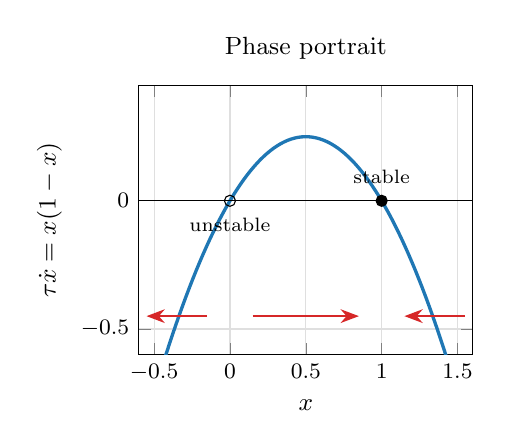
\begin{tikzpicture}
\begin{axis}[width=0.48\textwidth, height=5cm, xmin=-0.6, xmax=1.6, ymin=-0.6, ymax=0.45,
  xlabel={$x$}, ylabel={$\tau\dot x = x(1 - x)$}, title={Phase portrait}]
  \addplot[cA, very thick, domain=-0.6:1.6, samples=100] {x*(1-x)};
  \addplot[black, domain=-0.6:1.6, samples=2] {0};
  \addplot[only marks, mark=*, black] coordinates {(1,0)};
  \addplot[only marks, mark=o, black, mark options={fill=white}] coordinates {(0,0)};
  \draw[-{Stealth}, thick, cD] (axis cs:-0.15,-0.45) -- (axis cs:-0.55,-0.45);
  \draw[-{Stealth}, thick, cD] (axis cs:0.15,-0.45) -- (axis cs:0.85,-0.45);
  \draw[-{Stealth}, thick, cD] (axis cs:1.55,-0.45) -- (axis cs:1.15,-0.45);
  \node[font=\scriptsize, anchor=south] at (axis cs:1,0.03) {stable};
  \node[font=\scriptsize, anchor=north] at (axis cs:0,-0.03) {unstable};
\end{axis}
\end{tikzpicture}\hfill
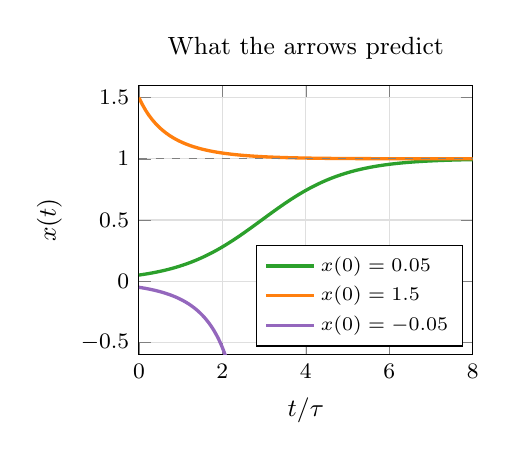
\begin{tikzpicture}
\begin{axis}[width=0.48\textwidth, height=5cm, xmin=0, xmax=8, ymin=-0.6, ymax=1.6,
  xlabel={$t/\tau$}, ylabel={$x(t)$}, title={What the arrows predict}, legend pos=south east, legend cell align=left]
  \addplot[cC, very thick, domain=0:8, samples=100] {0.05*exp(x)/(1-0.05+0.05*exp(x))};
  \addplot[cB, very thick, domain=0:8, samples=100] {1.5*exp(x)/(1-1.5+1.5*exp(x))};
  \addplot[cE, very thick, domain=0:2.9, samples=100] {-0.05*exp(x)/(1+0.05-0.05*exp(x))};
  \addplot[gray, dashed, domain=0:8, samples=2, forget plot] {1};
  \legend{$x(0) = 0.05$, $x(0) = 1.5$, $x(0) = -0.05$}
\end{axis}
\end{tikzpicture}
\end{center}

\textbf{Why the slope decides stability.} Near an equilibrium the curve is almost a straight line, $\phi(x) \approx \phi'(x^*)(x - x^*)$. A small nudge $\delta = x - x^*$ then obeys $\dot\delta = \phi'(x^*)\,\delta$, so $\delta(t) = \delta_0 e^{\phi'(x^*)t}$: it shrinks when the slope is negative and grows when it is positive. This is the one-dimensional version of the lecture's rule about the eigenvalues of the Jacobian.

\textbf{Why only stable equilibria matter in neurons.} Spike noise is constantly nudging the state, so a network can only rest at a stable equilibrium. An unstable one is a dividing line between outcomes, not a resting place.

\textbf{Two ideas that tests like.}
\begin{itemize}
\item \emph{The input shifts the curve.} $u$ adds a constant to $\phi$, moving the curve up or down. Two equilibria can move together, merge, and disappear. After that, the state has nowhere to stop. For Lecture 6's $f(x) = x^2$ this happens at $u = 1/4$.
\item \emph{Two stable equilibria with an unstable one between them make a memory.} Where the state ends up depends on which side of the unstable point it started, not on the current input. The network stores one bit.
\end{itemize}

%=====================================================================
\section{Designing a system: $A' = \tau A + I$, $B' = \tau B$}

Now turn it around. Given a target $\dot x = Ax + Bu$, choose what to feed the synapse.

\textbf{The problem.} An ideal implementation computes $Ax + Bu$ and passes it through a perfect integrator. Neurons have no perfect integrator, only the leaky synapse of Section~1. Feeding it $Ax + Bu$ directly gives the wrong system: the leak is added, and everything is scaled by $1/\tau$.

\textbf{The idea.} Feed the synapse $z = A'x + B'u$ instead: $A'x$ from a recurrent connection and $B'u$ from the input connection. Then choose $A'$ and $B'$ so the loop behaves exactly like the target.

\textbf{The derivation.} The loop equation with this $z$:
\[
\tau\dot x = A'x + B'u - x .
\]
To compare with $Ax$, the two $x$ terms must be combined into one matrix times $x$. You cannot write $(A' - 1)x$, because $A'$ is a matrix and $1$ is a number. Write the lone $x$ as $Ix$, since the identity leaves every vector unchanged:
\[
A'x - x = A'x - Ix = (A' - I)x \quad\Longrightarrow\quad \dot x = \frac{A' - I}{\tau}\,x + \frac{B'}{\tau}\,u .
\]
Matching coefficients with $\dot x = Ax + Bu$:
\[
\boxed{\ A' = \tau A + I, \qquad B' = \tau B\ }
\]
In 2-D, $A'x - x$ subtracts $x_1$ from the first row and $x_2$ from the second, which is why the $-1$'s land only on the diagonal: each component leaks only from itself. In 1-D, $I$ is just the number $1$.

\begin{center}
\begin{tabular}{@{}p{0.18\textwidth}p{0.74\textwidth}@{}}
\toprule
Piece & What it does \\
\midrule
$+I$ & Feeds the current state back to cancel the synapse's leak. It is the $-x$ term carried through the algebra. \\
$\times\tau$ & $A$ and $B$ are rates (units of 1/s). The synapse moves at (input $-$ state)$/\tau$ per second, so to move at rate $Ax + Bu$ its input must be $\tau$ times larger. It also makes $A'$, $B'$ dimensionless, as a Nengo \texttt{transform} needs. \\
which $\tau$ & The synapse on the \emph{recurrent} connection. \\
\bottomrule
\end{tabular}
\end{center}

In Nengo, the input connection is \texttt{Connection(u, x, transform=B', synapse=tau)} and the recurrent one is \texttt{Connection(x, x, transform=A', synapse=tau)}.

\textbf{Worked example} (not from the ramp): $\dot x = -2x + 4u$ with $\tau = 0.1$ s. Then $A' = 0.1(-2) + 1 = 0.8$ and $B' = 0.4$.
\begin{itemize}
\item \emph{Steady-state check.} Ideal: $\dot x = 0$ gives $x = 2u$. Neural: at rest the synapse's output equals its input, $x = 0.8x + 0.4u$, so $x = 2u$. They match.
\item \emph{Speed check.} $\tau_{\mathrm{eff}} = \tau/(1 - A') = 0.1/0.2 = 0.5$ s, which equals $1/|A|$. They match.
\end{itemize}

\textbf{Reading $A'$ backwards.} In 1-D, $A = (A' - 1)/\tau$. So $A' = 1$ is a perfect memory, $A' < 1$ leaks with $\tau_{\mathrm{eff}} = \tau/(1 - A')$, and $A' > 1$ explodes. This is Section~3 again with $k = A'$.

\textbf{The network can be faster than its synapses.} A low-pass filter with $\tau_d$ shorter than $\tau$ needs $A' = 1 - \tau/\tau_d < 0$. Strong negative feedback plus a large input gain speeds the loop up beyond any single synapse.

%=====================================================================
\section{The ideal answer of an integrator}

For $\dot x = u$ from $x(0) = 0$, the ideal state is the running area under the input, $x(t) = \int_0^t u(t')\,dt'$. Three rules make it easy to sketch:
\begin{itemize}
\item The \textbf{slope} of $x$ equals the current value of $u$.
\item When $u = 0$, $x$ \textbf{holds}. It does not fall back to zero; that is the memory.
\item Each piece \textbf{starts where the previous one ended}. There is no ``$+C$''.
\end{itemize}
\textbf{The process.} For each region, split the integral at the switching times; only stretches with $u \ne 0$ contribute. Example: $u = 3$ on $0.5 \le t < 1.5$, else $0$.
\[
x(t) = \begin{cases} 0, & t < 0.5,\\ \int_{0.5}^{t} 3\,dt' = 3(t - 0.5), & 0.5 \le t < 1.5,\\ \int_{0.5}^{1.5} 3\,dt' = 3, & t \ge 1.5. \end{cases}
\]
Check continuity at every switch (an integral cannot jump), and check that the final value is the pulse's area, height times width.

\begin{trap}
\textbf{The radius.} The ideal integral may exceed the radius, but the neural state cannot. Once the neurons saturate, the extra area is lost. When the input reverses, the state comes down by the full integral starting from the clipped value, so it ends up permanently offset below the ideal. For $u = 3\sin 3t$ with radius $1$, the ideal is $1 - \cos 3t \in [0, 2]$; after the first clip the neural state follows about $-\cos 3t$.
\end{trap}

%=====================================================================
\section{Why a neural integrator drifts}

For an integrator the recurrent connection should feed back exactly $x$. Neurons only approximate it: the decoder gives $\hat f(x) = x + \mathrm{error}(x)$. Put that into the loop with no input:
\[
\tau\dot x = \hat f(x) - x = \mathrm{error}(x).
\]
\begin{key}
The integrator's velocity is its own decoding error. Plotting $\mathrm{error}(x)/\tau$ against $x$ gives a Section~4 phase portrait: a wiggly curve near zero with many small stable and unstable zeros. With no input, the state slides to the nearest stable zero.
\end{key}

\begin{center}
\begin{tikzpicture}
\begin{axis}[width=0.88\textwidth, height=5cm, xmin=-1, xmax=1, ymin=-0.85, ymax=0.85,
  xlabel={represented value $x$}, ylabel={$\dot x$ (s$^{-1}$)}, xtick={-1,-0.8,...,1},
  title={Measured in Nengo: 30-neuron rate integrator, $\tau = 0.1$ s, no input}]
  \addplot[black, thick, domain=-1:1, samples=2] {0};
  \addplot[blue!70!black, very thick] table[x=x, y=phi] {pn3_data/neural_phase.dat};
  \addplot[only marks, mark=*, black] coordinates {(-0.898,0) (-0.748,0) (-0.005,0) (0.159,0) (0.371,0) (0.756,0)};
  \addplot[only marks, mark=o, black, mark options={fill=white}] coordinates {(-0.821,0) (-0.477,0) (0.013,0) (0.231,0) (0.509,0)};
\end{axis}
\end{tikzpicture}
\end{center}

\begin{center}
\begin{tabular}{@{}p{0.27\textwidth}p{0.33\textwidth}p{0.32\textwidth}@{}}
\toprule
Error source & Effect on the loop & What you see \\
\midrule
Static distortion (the decoder's fit is not perfect) & The fixed wiggly $\mathrm{error}(x)$ above & A smooth drift to the same place on every run \\
Spike noise ($z$ fluctuates spike by spike) & Random kicks to the state & A random walk: each run ends somewhere different \\
\bottomrule
\end{tabular}
\end{center}
Rate mode removes the spike noise but keeps the distortion. More neurons shrink both (distortion roughly as $1/n$, noise roughly as $1/\sqrt n$ in RMSE), so the drift slows, but it never stops completely.

%=====================================================================
\section{Unequal input and recurrent synapses}

PN3 uses a fast synapse on the input ($\tin = 5$ ms) and a slow one on the recurrence ($\tau = 50$ ms), and computes $A' = 1$, $B' = \tau$ with the slow one. What changes?

\subsection*{The intuitive picture: split the state in two}

Each synapse has its own output, and the population represents their sum:
\begin{itemize}
\item $p$, the output of the \textbf{input} synapse. It chases $\tau u$ quickly: $\tin\dot p = \tau u - p$.
\item $r$, the output of the \textbf{recurrent} synapse. It chases $x$ slowly: $\tau\dot r = x - r$.
\item The state is $x = r + p$.
\end{itemize}
Substituting $x = r + p$ into the recurrent equation:
\[
\tau\dot r = (r + p) - r = p \quad\Longrightarrow\quad \dot r = \frac{p}{\tau}.
\]
So the recurrent synapse integrates whatever the input synapse delivers. The input synapse is fast, so after a few $\tin$, $p \approx \tau u$, and then $\dot r \approx u$:
\[
x = r + p \;\approx\; \underbrace{\int_0^t u}_{r:\ \text{stored}} \;+\; \underbrace{\tau u}_{p:\ \text{in transit}} .
\]

\begin{howto}
With \emph{equal} synapses, the input's push $\tau u$ goes through the same slow synapse as the feedback, so it enters the state only gradually, at rate $u$. With a \emph{fast} input synapse, the full push $\tau u$ appears in the state almost at once, on top of the stored integral. The population represents both parts, so the decoded value includes both.
\end{howto}

\subsection*{The exact result}

The approximation $p \approx \tau u$ ignores the first few $\tin$, and $r$ really integrates the slightly delayed $p$. Accounting for that removes $\tin u$ from the lump:
\[
\boxed{\ x(t) = \int_0^t u \;+\; (\tau - \tin)\,(h_{\tin} * u)(t)\ }
\]
where $h_{\tin} * u$ is just $u$ smoothed by the fast synapse.

\subsection*{The Laplace derivation}

Each connection gets its own filter:
\[
X = \frac{1}{1 + s\tau}\,X + \frac{1}{1 + s\tin}\,\tau U .
\]
\begin{enumerate}
\item Collect the $X$ terms: $X\bigl(1 - \frac{1}{1 + s\tau}\bigr) = X\,\frac{s\tau}{1 + s\tau}$.
\item Solve: $X\,\frac{s\tau}{1 + s\tau} = \frac{\tau U}{1 + s\tin}$, so $X = \frac{1 + s\tau}{1 + s\tin}\cdot\frac{U}{s}$.
\item Split the ratio: $\frac{1 + s\tau}{1 + s\tin} = 1 + \frac{s(\tau - \tin)}{1 + s\tin}$.
\item Multiply by $U/s$; in the second term the $s$ cancels the $1/s$:
\[
X = \underbrace{\frac{U}{s}}_{\int u} + \underbrace{(\tau - \tin)\frac{U}{1 + s\tin}}_{(\tau - \tin)(h_{\tin} * u)} .
\]
\end{enumerate}
Same result as the intuitive picture, reached by algebra.

\subsection*{What it looks like}

Example (not from the ramp): $\tau = 0.1$ s, $\tin = 0.01$ s, $u = 2$ on $0 \le t < 0.5$, then $0$. The lump is about $(0.1 - 0.01)\times 2 = 0.18$.
\begin{center}
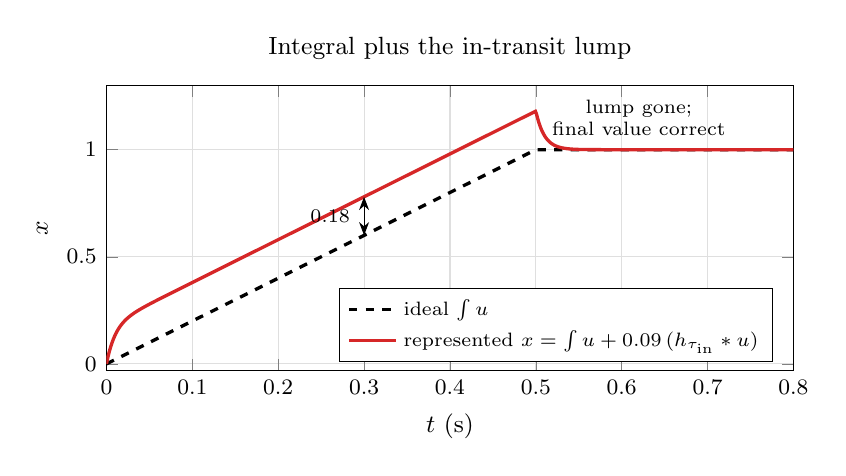
\begin{tikzpicture}
\begin{axis}[width=0.85\textwidth, height=5.2cm, xmin=0, xmax=0.8, ymin=-0.03, ymax=1.3,
  xlabel={$t$ (s)}, ylabel={$x$}, legend pos=south east, legend cell align=left,
  title={Integral plus the in-transit lump}]
  \addplot[black, very thick, dashed] coordinates {(0,0) (0.5,1) (0.8,1)};
  \addplot[cD, very thick, domain=0:0.8, samples=600]
    {(x<0.5)*(2*x + 0.09*2*(1-exp(-x/0.01))) + (x>=0.5)*(1 + 0.09*2*(1-exp(-50))*exp(-(x-0.5)/0.01))};
  \legend{ideal $\int u$, represented $x = \int u + 0.09\,(h_{\tin} * u)$}
  \draw[{Stealth}-{Stealth}] (axis cs:0.3,0.6) -- (axis cs:0.3,0.78);
  \node[font=\scriptsize, anchor=east] at (axis cs:0.295,0.69) {$0.18$};
  \node[font=\scriptsize, anchor=south, align=center] at (axis cs:0.62,1.02) {lump gone;\\final value correct};
\end{axis}
\end{tikzpicture}
\end{center}

\textbf{Sanity checks.}
\begin{itemize}
\item $\tin = \tau$: the lump is zero, and the perfect integrator returns.
\item The final value is unaffected: the lump exists only while $u \ne 0$.
\item The lump is set by $\tau - \tin \approx \tau$, not by $\tin$. A 5 ms input synapse does not just cause a 5 ms lag.
\end{itemize}

\textbf{For PN3 \S4.} The integral stays correct, but while the input is on the trace sits about $(\tau - \tin)u = 0.045 \times 0.9 \approx 0.04$ above the ideal, and it snaps back when the input stops. For ramp and sine inputs the lump follows $u$, so the trace looks slightly \emph{ahead} of the ideal.

%=====================================================================
\section{Leaky integrators, and why integrators are fragile}

If the feedback is slightly less than $x$, $z = A'x$ with $A'$ just below $1$, then $\tau\dot x = -(1 - A')x$. Part of the leak survives, and the state decays with
\[
\tau_{\mathrm{eff}} = \frac{\tau}{1 - A'} .
\]
Because this divides by a small number, memory is extremely sensitive to the feedback gain. With $\tau = 50$ ms: $A' = 0.99$ gives $5$ s, $A' = 0.999$ gives $50$ s, and $A' = 1.01$ grows until saturation. A $1\%$ decoder error can change the memory time tenfold, which is why accurate neural integrators need many neurons.

Biology uses the leak deliberately. The horizontal eye-position circuit drifts back to centre with $\tau_{\mathrm{eye}} \approx 70$ s, so it is modelled as $\dot x = -x/\tau_{\mathrm{eye}} + v$, implemented with $A' = 1 - \tau/\tau_{\mathrm{eye}}$ and $B' = \tau$.

%=====================================================================
\section{The oscillator: a loop that rotates}

With a 2-D state and $A = \begin{pmatrix} 0 & -\omega \\ \omega & 0 \end{pmatrix}$, the velocity $Ax$ is always perpendicular to the position $x$. Anything whose velocity is always at right angles to where it is goes round in a circle, here at $\omega$ rad/s.

Read $A' = I + \tau A = \begin{pmatrix} 1 & -\tau\omega \\ \tau\omega & 1 \end{pmatrix}$ as: keep the current state ($I$), plus a small sideways nudge ($\tau A$). Each pass round the loop rotates the state a little.
\begin{itemize}
\item \textbf{It needs a kick.} At the origin $Ax = 0$, so nothing moves until an input pushes the state off zero.
\item \textbf{The neurons set the amplitude.} The ideal oscillator keeps whatever amplitude the kick gave it. The neural one is bounded by the radius, and noise or distortion can make it shrink to zero.
\item \textbf{High frequencies are harder.} A large $\tau\omega$ means each pass must produce a big rotation, so decoding errors and the synapse's approximations matter more. That is why a Nengo oscillator tracks worse as the frequency rises.
\end{itemize}
A damped oscillator adds $-\gamma$ on the diagonal of $A$; then $A'$ has $1 - \tau\gamma$ on its diagonal and the trajectory spirals inward.

%=====================================================================
\section{Nonlinear systems, and the controlled integrator}

\textbf{Same recipe, with functions.} Nothing in Section~5 needed $z$ to be linear. For $\dot x = f(x) + g(u)$, feed the synapse
\[
f'(x) = \tau f(x) + x, \qquad g'(u) = \tau g(u):
\]
the same two moves, scale the desired rate by $\tau$ and add $x$ to cancel the leak. In Nengo the recurrent connection gets \texttt{function=}. If $f$ multiplies state variables together (like $x_1x_2$), one population must represent all of them together, as with $xy$ in Test~2. The Lorenz attractor is one 3-D population for that reason, and it needs no kick because its origin is not an equilibrium.

\textbf{The controlled integrator: a memory with a knob.} Target $\dot x = c\,x + u$, where $c(t)$ is itself an input. Here $c$ plays the role of the leak, and you can turn it while the network runs: $c = 0$ integrates, $c < 0$ forgets with time constant $1/|c|$, and $c > 0$ grows. Effectively the recurrent gain becomes $1 + \tau c$. The feedback $f'(x, c) = x + \tau c x$ contains the product $cx$, so one 2-D population represents $(x, c)$ together. Only the $x$ component is fed back; $c$ enters dimension 2 through its own connection, with no recurrence on it.

%=====================================================================
\newpage
\section{One-page summary}

\begin{key}
\textbf{When a question looks unfamiliar:} write $\tau\dot x = z - x$, decide what $z$ is (everything fed into the synapse), and simplify. Then either read the behaviour off the sign of $\dot x$ (phase portrait), or match coefficients with the target system.
\end{key}

\begin{center}
\renewcommand{\arraystretch}{1.25}
\begin{tabular}{@{}p{0.2\textwidth}p{0.28\textwidth}p{0.44\textwidth}@{}}
\toprule
Topic & What $z$ is & What to remember \\
\midrule
Synapse & any input & $\tau\dot y = z - y$: chases its input, leaks with $\tau$ \\
Loop & $g(u) + f(x)$ & $\tau\dot x = g(u) + f(x) - x$; $x = g + f$ is only the steady state \\
Linear feedback & $u + kx$ & Left-over leak $1 - k$: forget, remember ($k = 1$), explode \\
Phase portrait & $u + f(x)$ & Zeros are equilibria; downward crossing is stable; follow the arrows \\
Design & $A'x + B'u$ & $A' = \tau A + I$, $B' = \tau B$, recurrent $\tau$; check steady state and speed \\
Ideal integral & $x + \tau u$ & Slope $= u$, holds when $u = 0$, no $+C$, watch the radius \\
Drift & $x + \mathrm{error}(x)$ & Distortion drifts the same way each run; noise random-walks \\
Unequal synapses & $x$ (slow) $+ \tau u$ (fast) & $\int u + (\tau - \tin)(h_{\tin} * u)$; final value correct \\
Leaky integrator & $A'x$, $A' \approx 1$ & $\tau_{\mathrm{eff}} = \tau/(1 - A')$: extremely sensitive \\
Oscillator & $(I + \tau A)x$ & Rotation; needs a kick; radius bounds the amplitude \\
Nonlinear & $\tau f(x) + x + \tau g(u)$ & Same recipe with functions; products need one joint population \\
Controlled integrator & $x + \tau c x + \tau u$ & Adjustable leak; 2-D population representing $(x, c)$ \\
\bottomrule
\end{tabular}
\end{center}

\end{document}
